\documentclass[10pt,letterpaper]{article}

\usepackage[utf8]{inputenc}
\usepackage[T1]{fontenc}
\usepackage[letterpaper,top=0.82in,bottom=0.82in,left=0.84in,right=0.84in]{geometry}
\usepackage{lmodern}
\usepackage[scaled=0.86]{inconsolata}
\usepackage{microtype}
\usepackage{xcolor}
\usepackage{graphicx}
\usepackage{booktabs}
\usepackage{tabularx}
\usepackage{array}
\usepackage{enumitem}
\usepackage{amsmath}
\usepackage{amssymb}
\usepackage{tcolorbox}
\usepackage{fancyhdr}
\usepackage{lastpage}
\usepackage{titlesec}
\usepackage{caption}
\usepackage{hyperref}

% ---- Zeus Editorial Palette Tokens ----
\definecolor{zeusPaper}{HTML}{F7F4EC}
\definecolor{zeusNight}{HTML}{0C0F16}
\definecolor{zeusInk}{HTML}{11151C}
\definecolor{zeusGraphite}{HTML}{4A5260}
\definecolor{zeusMuted}{HTML}{78808F}
\definecolor{zeusBolt}{HTML}{D93B21}
\definecolor{zeusBoltSoft}{HTML}{FCEBE8}
\definecolor{zeusTeal}{HTML}{156654}
\definecolor{zeusTealSoft}{HTML}{E5F3EF}
\definecolor{zeusSlate}{HTML}{28527D}
\definecolor{zeusSlateSoft}{HTML}{EBF1F8}
\definecolor{zeusOchre}{HTML}{B5760D}
\definecolor{zeusPanel}{HTML}{EFECE3}
\definecolor{zeusRule}{HTML}{D8D2C5}

\hypersetup{
  colorlinks=true,
  linkcolor=zeusSlate,
  citecolor=zeusTeal,
  urlcolor=zeusSlate,
  pdftitle={Zeus: Bounded Concurrency and Fail-Closed Authority for Verifiable Agentic Coding},
  pdfauthor={Vikram Viswanath},
  pdfsubject={Systems Technical Report TR-01}
}

\captionsetup{
  font={small},
  labelfont={bf,sf,color=zeusBolt},
  textfont={color=zeusInk},
  justification=raggedright,
  singlelinecheck=false,
  skip=5pt
}

% ---- Section & Header Styling ----
\titleformat{\section}
  {\large\sffamily\bfseries\color{zeusInk}}
  {\color{zeusBolt}\thesection.}{0.55em}{}
  [\vspace{2pt}{\color{zeusRule}\titlerule[0.6pt]}]

\titleformat{\subsection}
  {\normalsize\sffamily\bfseries\color{zeusSlate}}
  {\thesubsection}{0.55em}{}

\titlespacing*{\section}{0pt}{13pt}{6pt}
\titlespacing*{\subsection}{0pt}{9pt}{4pt}

\pagestyle{fancy}
\setlength{\headheight}{19pt}
\fancyhf{}
\renewcommand{\headrulewidth}{0.5pt}
\renewcommand{\headrule}{\hbox to\headwidth{\color{zeusRule}\leaders\hrule height \headrulewidth\hfill}}
\fancyhead[L]{\footnotesize\sffamily\color{zeusMuted}ZEUS TECHNICAL REPORT TR-01}
\fancyhead[R]{\footnotesize\ttfamily\color{zeusMuted}HEAD 9dbba43 $\cdot$ github.com/vikramwish/zeus}
\fancyfoot[C]{\footnotesize\sffamily\color{zeusMuted}Page \thepage\ of \pageref{LastPage}}

\tcbuselibrary{skins,breakable}
\newtcolorbox{invariantbox}[1][]{
  enhanced,
  breakable,
  colback=zeusPanel,
  colframe=zeusRule,
  borderline west={2.4pt}{0pt}{zeusTeal},
  boxrule=0.6pt,
  arc=3pt,
  left=10pt,
  right=10pt,
  top=7pt,
  bottom=7pt,
  fonttitle=\sffamily\bfseries\small\color{zeusTeal},
  title=#1
}

\newtcolorbox{caveatbox}[1][]{
  enhanced,
  breakable,
  colback=zeusBoltSoft,
  colframe=zeusRule,
  borderline west={2.4pt}{0pt}{zeusBolt},
  boxrule=0.6pt,
  arc=3pt,
  left=10pt,
  right=10pt,
  top=7pt,
  bottom=7pt,
  fonttitle=\sffamily\bfseries\small\color{zeusBolt},
  title=#1
}

\newcommand{\code}[1]{\textnormal{\small\ttfamily #1}}
\newcolumntype{L}{>{\raggedright\arraybackslash}X}

\setlength{\parindent}{0pt}
\setlength{\parskip}{5.5pt}

\begin{document}
\thispagestyle{empty}

% ---- Masthead Banner ----
\noindent
\begin{tcolorbox}[
  enhanced,
  colback=zeusNight,
  colframe=zeusNight,
  arc=5pt,
  left=14pt,
  right=14pt,
  top=12pt,
  bottom=12pt
]
  {\footnotesize\ttfamily\bfseries\color{zeusBolt} TECHNICAL REPORT TR-01 \hfill SYSTEMS, CONCURRENCY \& VERIFICATION}\\[3pt]
  {\color{white!30!zeusNight}\rule{\linewidth}{0.5pt}}\\[8pt]
  {\LARGE\sffamily\bfseries\color{white} Zeus: Bounded Concurrency and Fail-Closed Authority\\[2pt]
  for Verifiable Agentic Coding}\\[8pt]
  {\small\sffamily\color{zeusMuted} Author: Vikram Viswanath \quad$\cdot$\quad Repository Snapshot: \code{9dbba43} (2026-11-13) \quad$\cdot$\quad Implementation: 7,245 LOC Rust, 266 Tests}
\end{tcolorbox}

\vspace{4pt}
\begin{center}
  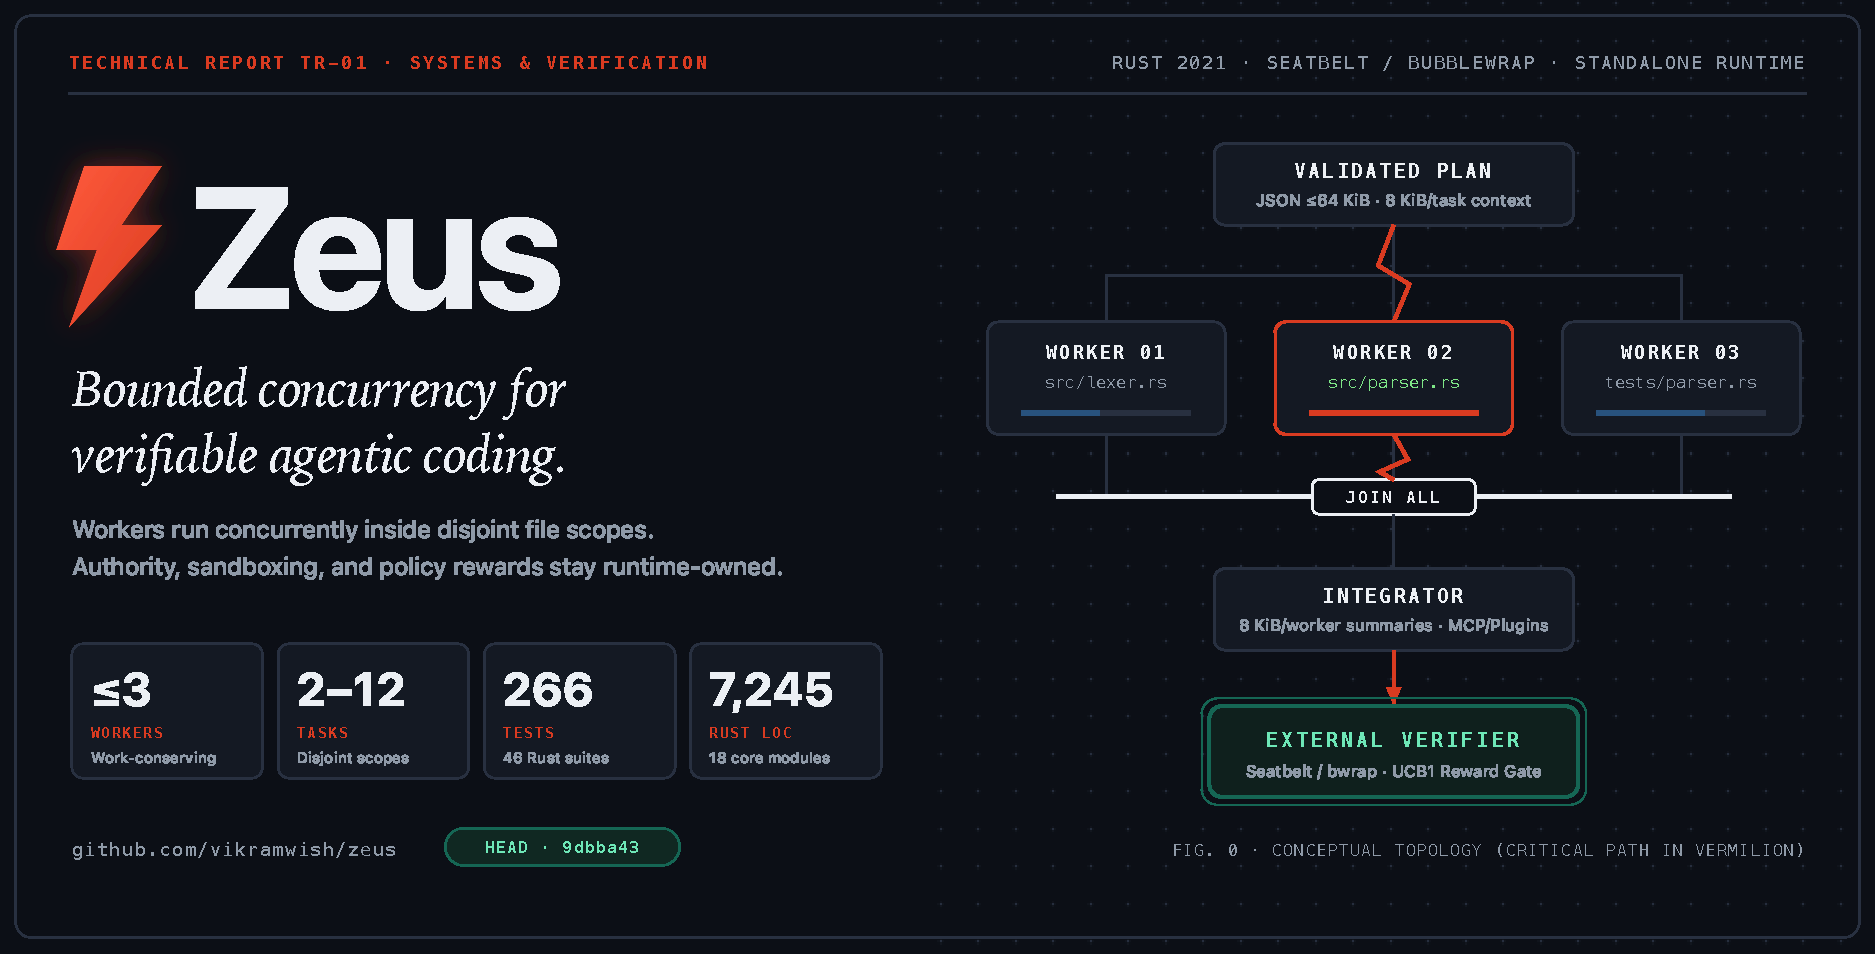
\includegraphics[width=0.96\textwidth]{figures/zeus-cover.pdf}
\end{center}
\vspace{1pt}

% ---- Abstract ----
\begin{tcolorbox}[
  enhanced,
  colback=zeusPanel,
  colframe=zeusRule,
  boxrule=0.6pt,
  arc=4pt,
  left=12pt,
  right=12pt,
  top=8pt,
  bottom=8pt
]
\textbf{\sffamily\color{zeusBolt} Abstract.}\quad
Autonomous coding agents routinely conflate natural-language model output with system authority: they allow generated tool requests to escape declared paths, waste multi-core capacity behind synchronous batch barriers, or corrupt adaptive routing state whenever transient network timeouts occur. \textbf{Zeus} is a standalone Rust runtime ($7{,}245$ lines across $18$ modules) that separates untrusted model reasoning from host capability enforcement, OS-level sandboxing, and verification-gated policy learning.

Zeus bounds parallel coding to $1$--$3$ workers executing over a work-conserving FIFO queue with global pre-admission scope checking, ensuring exact-file disjointness and fail-closed rejection before any worker thread spawns. Candidate mutations exclude secret-like files and expose zero write authority over the external verifier or state directory, which run inside macOS Seatbelt or Linux \code{bubblewrap} profiles. Strategy selection between a direct implementer and parallel workers uses a deterministic UCB1 contextual bandit updated \emph{strictly} on verified pass or verified fail outcomes, paired with an experimental shadow-only outcome scorer (\emph{Zeus Judge}) governed by eight abstention gates. The implementation is verified deterministically by $266$ static Rust tests across $46$ suites requiring no live LLM, and evaluated across $14$ exploratory local Qwen~3.5-9B field trials showing $0/10$ infrastructure errors contaminating routing tables.\\[5pt]
{\color{zeusRule}\rule{\linewidth}{0.5pt}}\\[4pt]
{\footnotesize\textbf{\sffamily\color{zeusSlate} Reproducibility Artifacts.}\quad
All figures render deterministically from Rust source \& test inspection plus \code{research/data/field\_runs.json} via \code{research/scripts/build\_figures.py}. Companion materials: \code{research/index.html} (interactive lab), \code{research/REPORT.md}, \code{DESIGN.md}, and \code{cargo test --locked} (rev.\ \code{9dbba43}).}
\end{tcolorbox}

\clearpage

% ==============================================================================
\section{Introduction and Threat Model}
\label{sec:intro}

Multi-step coding agents sit on an awkward fault line between stochastic token generators and deterministic operating-system side effects. When an agent edits a software repository, at least four failure modes routinely compound:
\begin{enumerate}[leftmargin=1.5em,itemsep=2pt,topsep=2pt]
  \item \textbf{Implicit capability elevation}: prompts suggest narrow tasks, while raw shell or path tools permit writes across adjacent tests, hidden secrets, or verifier harnesses.
  \item \textbf{Straggler-amplified concurrency}: parallel fan-out systems stall fast workers at coarse batch barriers or allow concurrent edits to race on the same files.
  \item \textbf{Biased online adaptation}: adaptive routers credit or penalize execution strategies when rate limits, deadlocked HTTP streams, or user cancellations abort a run before verification.
  \item \textbf{Unbounded transcript and handoff growth}: multi-worker aggregation or multi-turn file reads blow provider context windows, causing silent truncation or mid-run abandonment.
\end{enumerate}

Zeus (\code{github.com/vikramwish/zeus}) treats these failure modes as systems engineering invariants rather than prompt-engineering problems. Designed after direct inspection of local agent runtime ancestors (\emph{Hermes} revisions \code{bf0203a7} / \code{c419cf7c} and \emph{Prime} revisions \code{c4c238ca} / \code{c6d4da94}), Zeus is implemented from scratch in Rust~2021 (MSRV~1.85) with explicit dependency minimalism (\code{serde}, \code{serde\_json}, \code{ureq}, \code{sha2}, \code{libc}, \code{base64}, \code{ring}, \code{url}).

\begin{figure}[htbp]
  \centering
  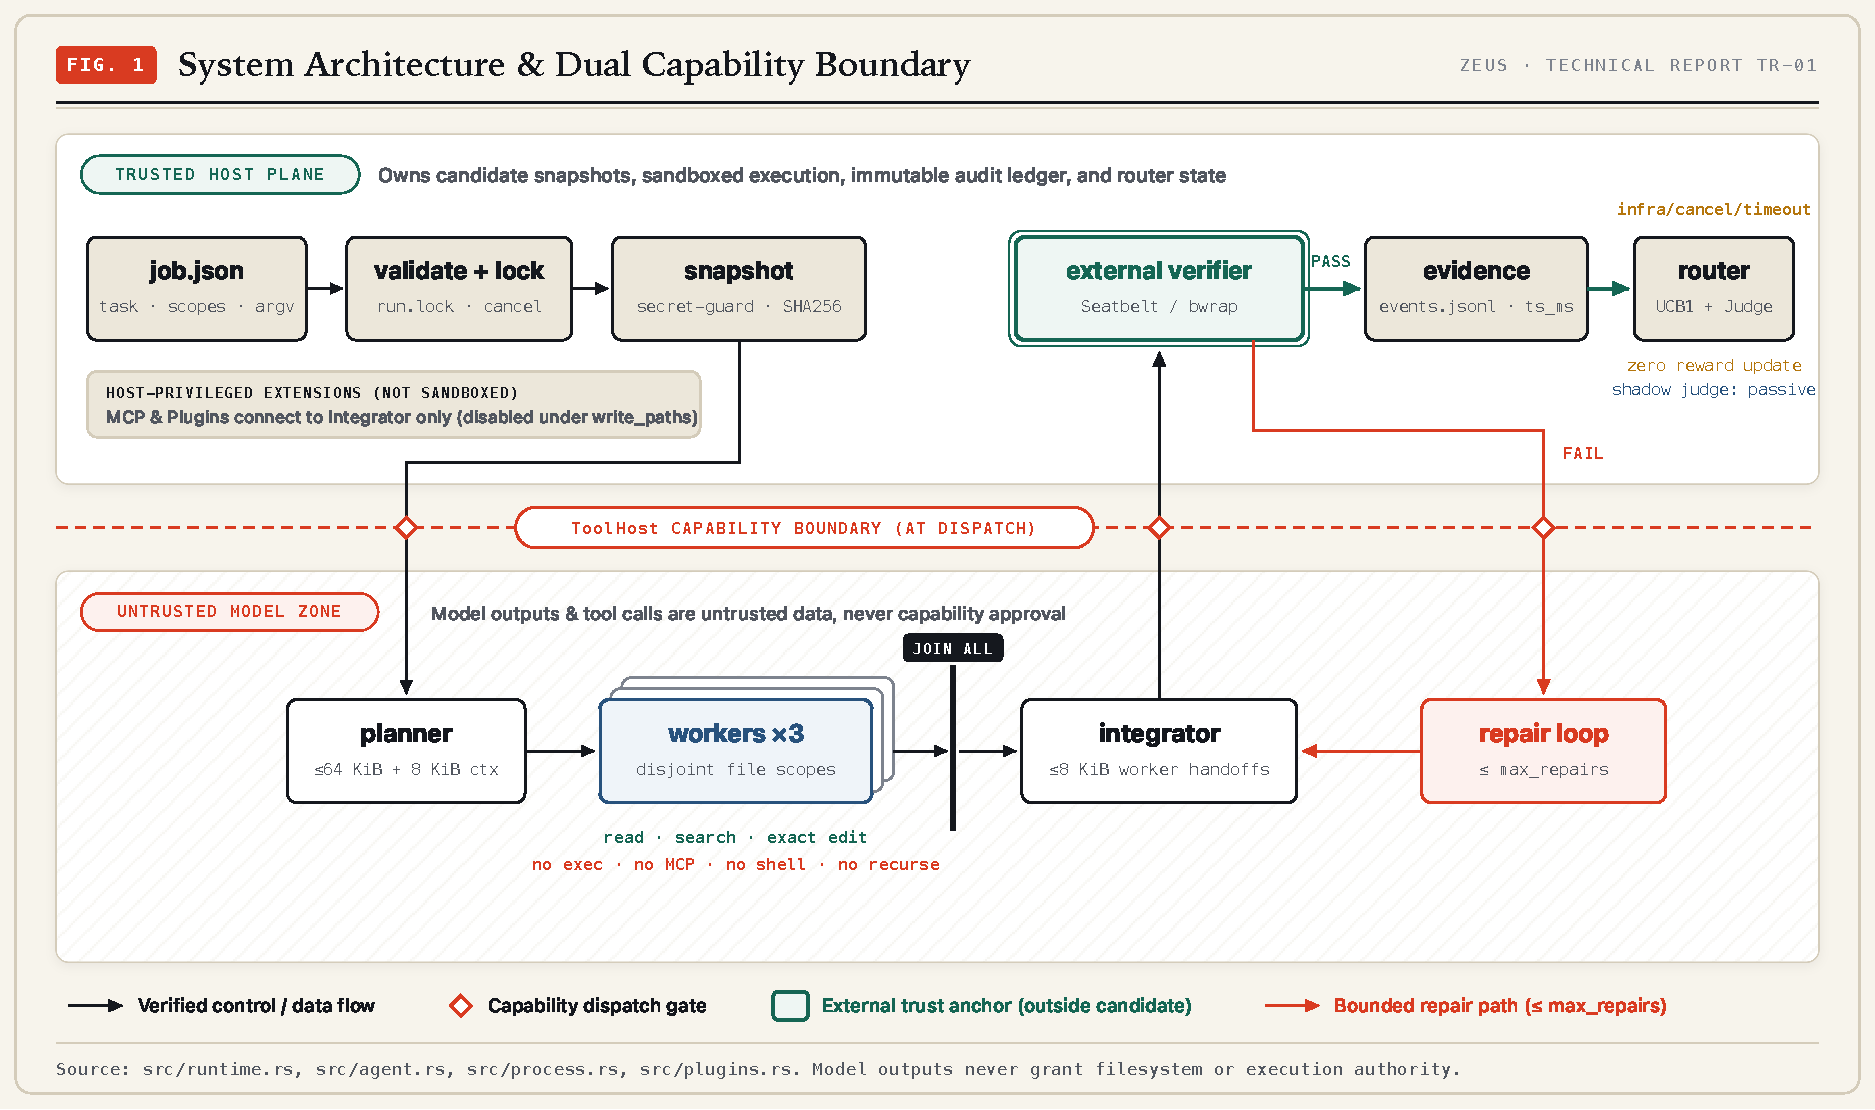
\includegraphics[width=\textwidth]{figures/fig1-system.pdf}
  \caption{Zeus dual capability boundary. Host orchestration, secret-excluding candidate snapshots, OS-sandboxed external verification, immutable audit logging, and UCB1/Judge state remain inside the trusted host plane, isolated from untrusted planner, worker, and integrator completions via \code{ToolHost} checks.}
  \label{fig:arch}
\end{figure}

Figure~\ref{fig:arch} illustrates the two-plane architecture. Every execution lifecycle splits cleanly at the \code{ToolHost} dispatch boundary:
\begin{itemize}[leftmargin=1.4em,itemsep=2pt,topsep=2pt]
  \item \textbf{Trusted Host Plane}: validates the CLI and \code{job.json}, acquires an exclusive \code{run.lock}, installs POSIX signal handlers without \code{SA\_RESTART}, clones the repository into a candidate workspace excluding VCS/build trees and secret-like files, executes the configured external verifier inside macOS Seatbelt or Linux \code{bubblewrap}, persists append-only \code{events.jsonl}, and commits verified routing updates via atomic write-\code{fsync}-rename.
  \item \textbf{Untrusted Model Zone}: hosts the planner (strict JSON $\le 64$\,KiB plus $\le 8$\,KiB per-task handoffs), $1$--$3$ concurrent file-scoped coding workers, an integrator consuming bounded $8$\,KiB worker handoffs, and a bounded repair loop ($\le$ \code{max\_repairs}, default $2$, ceiling $8$). No model token or tool argument is ever treated as a capability grant.
\end{itemize}

\begin{caveatbox}[Scope of Claims and Empirical Honesty]
Zeus is an early-working research prototype, not a benchmark-topping general software engineer. Deterministically passing tests verify runtime mechanics (protocol parsing, sandboxing, compaction, UCB1 math, abstention gates) against mocked servers and local fixtures. The $14$ empirical field trials reflect exploratory Qwen~3.5-9B development runs on an isolated Python key-value fixture rather than a held-out benchmark. Deterministic test execution exercises both macOS Seatbelt and Linux \code{bubblewrap} sandboxing end-to-end in CI, whereas exploratory Qwen~3.5-9B field trials ran on macOS.
\end{caveatbox}

% ==============================================================================
\section{Formal Runtime Architecture and Invariants}
\label{sec:invariants}

\subsection{Work-Conserving FIFO Admission}

Rather than dispatching tasks in fixed barrier waves of size $k$, \code{agent::run\_tasks} (\code{src/agent.rs}) maintains a shared \code{Mutex}-protected cursor over the validated queue $T_0, \dots, T_{m-1}$ serviced by $k \in \{1, 2, 3\}$ scoped worker threads (\code{std::thread::scope}). Each idle worker atomically pops the next unclaimed index $i$, executes until completion or failure, and writes its bounded result directly into slot $i$ of the output buffer.

\begin{figure}[htbp]
  \centering
  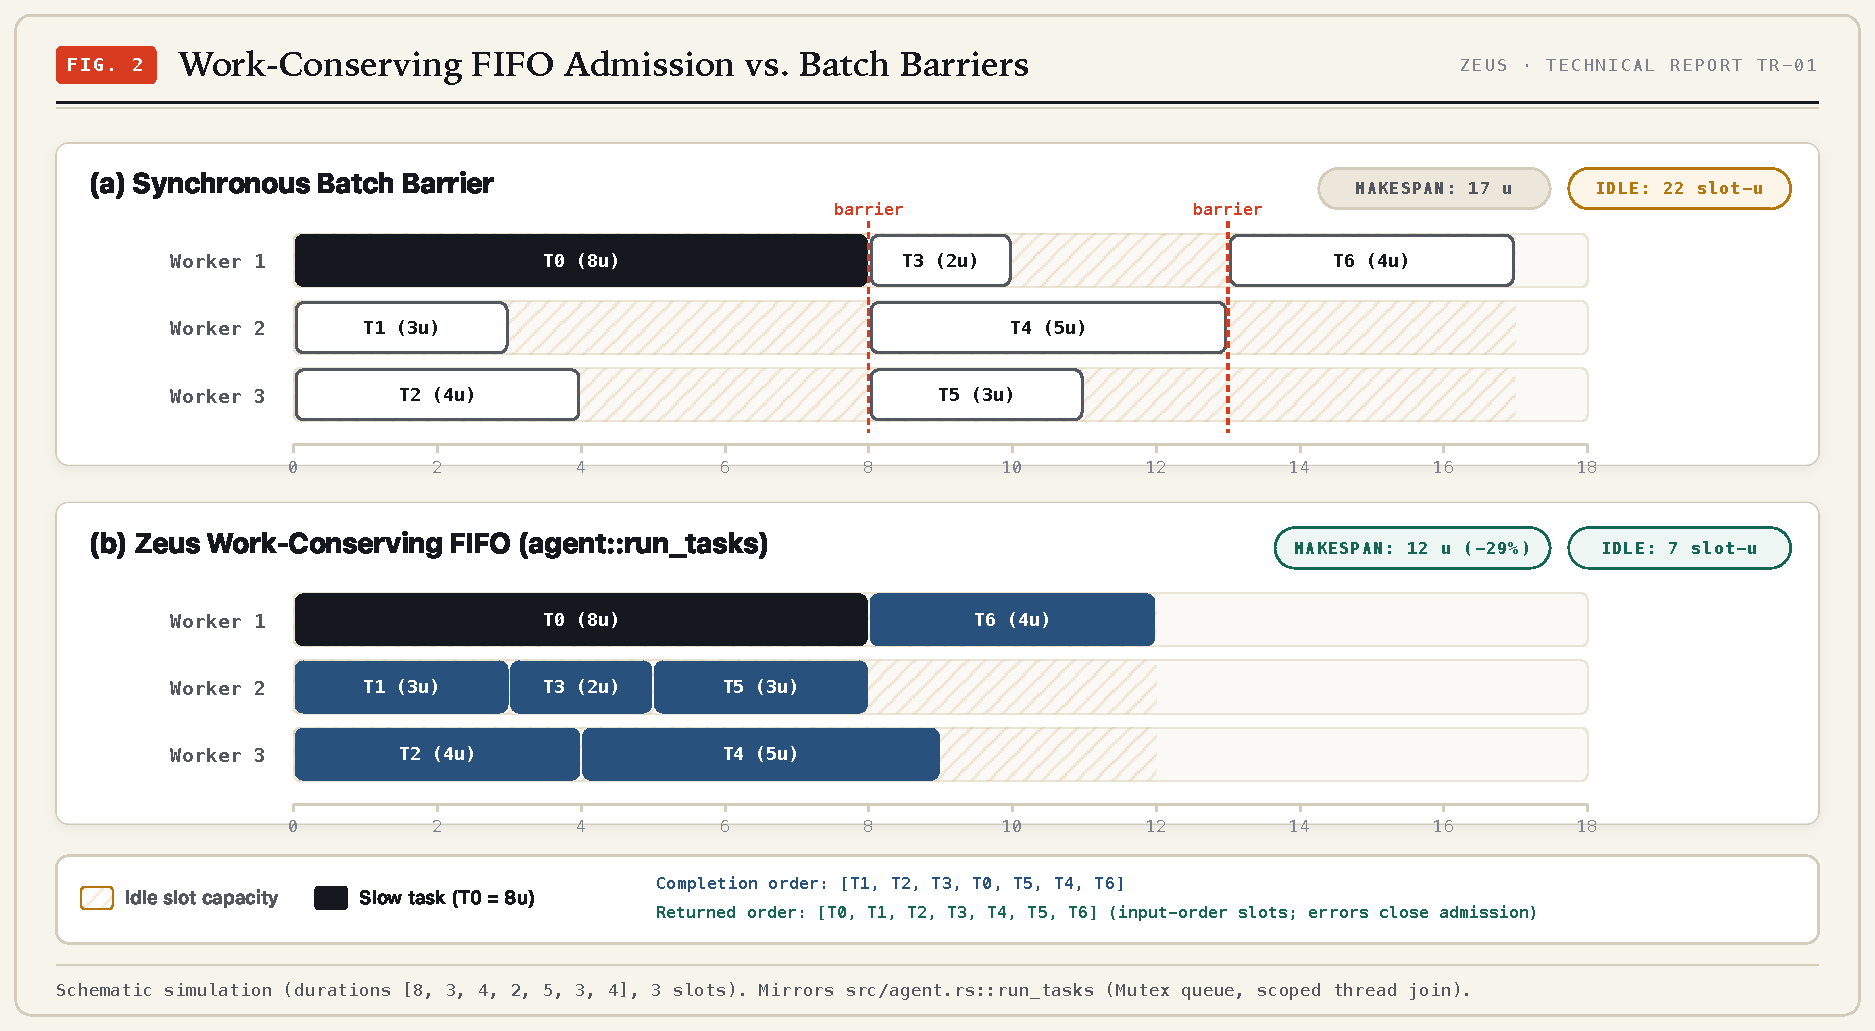
\includegraphics[width=\textwidth]{figures/fig2-scheduler.pdf}
  \caption{Comparison between synchronous batch barriers and Zeus work-conserving FIFO admission for illustrative task durations $[8,3,4,2,5,3,4]$ across $k=3$ workers. Fast workers refill immediately while output slots preserve planner declaration order.}
  \label{fig:scheduler}
\end{figure}

For deterministic heterogeneous workloads such as durations $d = [8, 3, 4, 2, 5, 3, 4]$ with $k = 3$ (Figure~\ref{fig:scheduler}), a synchronous batch barrier yields makespan $\sum_b \max_{t \in b} d_t = 8 + 5 + 4 = 17$\,u and $22$ idle slot-units, whereas list-scheduled FIFO admission lowers makespan to $12$\,u ($-29.4\%$) and idle capacity to $7$ slot-units ($-68.2\%$), bounded by Graham's classic greedy scheduling inequality $C_{\max} \le \frac{1}{k}\sum d_i + \frac{k-1}{k}\max d_i$. Upon any worker error, shared cancellation state closes new queue admissions immediately while running workers finish cleanly or abort on whole-job deadline/signal checks (\code{src/cancel.rs}).

\subsection{Pre-Admission Write-Scope Isolation}

Under parallel execution (\code{src/runtime.rs}), Zeus invokes a planner constrained to emit $2$--$12$ coding subtasks in a single JSON payload bounded at $64$\,KiB. Each subtask $T_i$ must supply a non-empty task description, a non-empty list of explicit file claims $W_i$, and an optional bounded handoff \code{context} string. Before any worker thread spawns, Zeus evaluates five whole-plan safety invariants across $\mathcal{P} = \{(T_i, W_i)\}_{i=1}^{m}$ (denoting path prefix by $\preceq$):

\begin{invariantbox}[Theorem 1 (Pre-Admission Disjointness \& Fail-Closed Containment)]
Let $p \in W_i$ be any claimed write path, let $\mathrm{norm}(p)$ denote its canonical ASCII lowercase form, and let $A \subseteq \Sigma^+$ be the optional \code{autonomy.write\_paths} allowlist ($\le 128$ entries). Plan $\mathcal{P}$ is admitted iff all five conditions hold simultaneously:
\begin{align}
\text{(Canonical Syntax)} \quad & \forall i, \forall p \in W_i:\; p \text{ is non-empty ASCII, } p_0 \ne \text{``/''},\; \text{``..''} \notin \mathrm{segs}(p),\; \text{``//''} \notin p, \\
\text{(Explicit Files)} \quad & \forall i:\; W_i \ne \emptyset \ \land\ \forall p \in W_i,\ p \text{ names an exact file (not a directory)}, \\
\text{(Global Disjointness)} \quad & \forall (i, p) \ne (j, q):\; \mathrm{norm}(p) \ne \mathrm{norm}(q) \ \land\ \mathrm{norm}(p) \not\preceq \mathrm{norm}(q), \\
\text{(Autonomy Subset)} \quad & A \ne \emptyset \implies \forall i, \forall p \in W_i:\; \exists a \in A \text{ s.t. } \mathrm{norm}(a) \preceq \mathrm{norm}(p), \\
\text{(Bounded Handoffs)} \quad & \forall i:\; |\mathrm{context}_i|_{\text{bytes}} \le 8192,\quad |\mathcal{P}_{\text{JSON}}|_{\text{bytes}} \le 65536.
\end{align}
Violation of any clause aborts the parallel plan with zero candidate mutations and zero spawned workers.
\end{invariantbox}

At runtime, candidate file writes additionally acquire \code{Workspace.mutation: Mutex<()>} (\code{src/workspace.rs}), perform SHA-256 content-hash checks against pre-read state for exact-edit fidelity, and enforce per-worker tool isolation: workers expose only read, search, and exact-edit primitives---no command execution, no MCP servers, no plugin tools, and no recursive delegation. Symlinks escaping the workspace root, excluded metadata directories, and files matching \code{secret\_like} heuristics (\code{PRIVATE KEY-----}, \code{sk-}, \code{AKIA}/\code{ASIA}, \code{ghp\_}--\code{ghs\_}, \code{xox*}, \code{AIza}, \code{.env}) are withheld before any model observes them (Figure~\ref{fig:ownership}).

\begin{figure}[htbp]
  \centering
  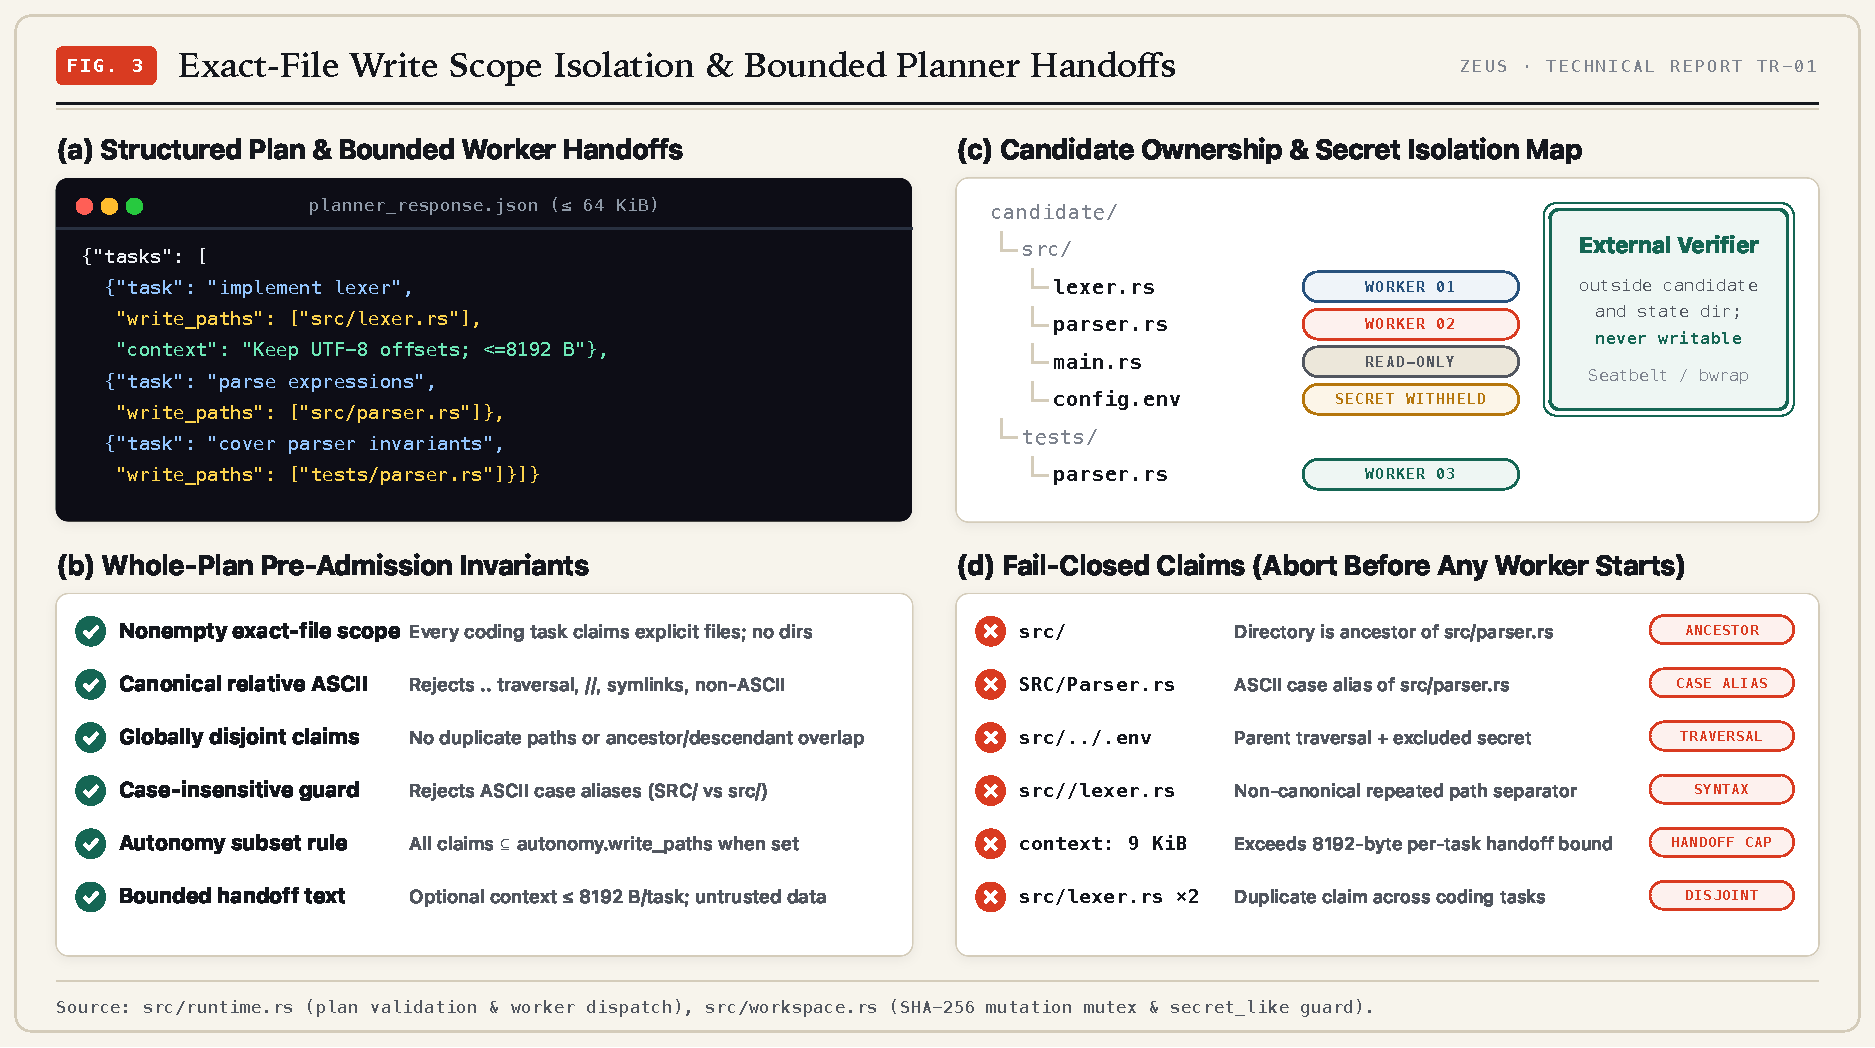
\includegraphics[width=\textwidth]{figures/fig3-ownership.pdf}
  \caption{Whole-plan pre-admission scope verification (\code{src/runtime.rs}, \code{src/workspace.rs}). Disjoint exact-file claims proceed concurrently while ancestor, ASCII case-alias, traversal, duplicate, and oversized handoff claims abort fail-closed prior to worker spawn.}
  \label{fig:ownership}
\end{figure}

\subsection{Sandboxed External Verification and Extensions Trust Model}

Verification runs outside both the model loop and candidate ownership assumptions (\code{src/process.rs}):
\begin{itemize}[leftmargin=1.4em,itemsep=2pt,topsep=2pt]
  \item \textbf{macOS Seatbelt}: denies default capabilities and restricts writes strictly to the candidate directory and an explicit scratch path while keeping source repository and state directories read-protected/unwritable.
  \item \textbf{Linux \code{bubblewrap}}: unshares PID and IPC namespaces (\code{--unshare-pid --unshare-ipc}), mounts procfs, binds the candidate tree read-write and host runtime paths read-only, drops environment secrets, and sets \code{--die-with-parent}.
  \item \textbf{Host-Privileged Extensions}: optional local MCP servers (\code{src/mcp.rs}) and manifest-v1 plugins (\code{src/plugins.rs}, opt-in via \code{--allow-plugins}, capped at $16$ plugins, $64$ tools, and $64$ skills) run on the host side rather than inside Seatbelt/bubblewrap. Accordingly, Zeus limits plugin and MCP exposure solely to the integrator (never sub-workers), automatically disables both when scoped \code{autonomy.write\_paths} are active, and re-runs the external verifier after any \code{run\_end} hook executes.
\end{itemize}

\begin{table}[htbp]
  \centering
  \small
  \caption{Core runtime memory, concurrency, and extension bounds enforced in code (\code{HEAD 9dbba43}).}
  \label{tab:bounds}
  \begin{tabularx}{\textwidth}{@{}llrL@{}}
    \toprule
    \textbf{Mechanism} & \textbf{Module} & \textbf{Hard Bound} & \textbf{Enforcement Behavior} \\
    \midrule
    Worker Concurrency & \code{src/runtime.rs} & $1 \le k \le 3$ & Work-conserving FIFO queue over $2$--$12$ coding subtasks \\
    Planner Response & \code{src/runtime.rs} & $\le 64$\,KiB JSON & Pre-admission validation rejects malformed or oversized plans \\
    Per-Task Planner Context & \code{src/runtime.rs} & $\le 8{,}192$\,B & Bounded hint string passed cleanly into worker prompt \\
    Worker Handoff Projection & \code{src/output.rs} & $\le 8{,}192$\,B / worker & $75\%$ head / $25\%$ tail + \code{[zeus: middle omitted]}; raw output in \code{events.jsonl} \\
    Transcript Compaction & \code{src/agent.rs} & $\ge 64$\,KiB ($1$\,MiB def.) & Elides old tool outputs (\code{\{"elided":true\}}); protects last $4$ results \\
    Tool Output & \code{src/agent.rs} & $256$\,KiB / $128$\,KiB & Truncates oversized tool reads; caps \code{process::capture} at $128$\,KiB \\
    Autonomy Guardrails & \code{docs/AUTONOMY.md} & $\le 128$ paths / $8$ repairs & Restricts write scope, repair rounds ($0$--$8$, def.\ $2$), and calls ($1$--$1024$) \\
    Snapshot Ingestion & \code{src/workspace.rs} & $2{,}000$ files / $64$\,MiB & Depth $\le 128$, per-file $\le 16$\,MiB; skips VCS/deps and secrets \\
    Extension Envelope & \code{src/plugins.rs} & $16$ plugins / $64$ tools & Disabled under \code{write\_paths}; triggers mandatory \code{run\_end} re-verification \\
    \bottomrule
  \end{tabularx}
\end{table}

% ==============================================================================
\section{Verifier-Anchored Bandit Routing}
\label{sec:routing}

For any coding context string $c$ ($\le 256$\,B, up to $1{,}024$ retained contexts per policy file saved atomically with \code{0o600} permissions), Zeus selects an execution strategy $a \in \{\text{Direct}, \text{Parallel}\}$ using deterministic UCB1 (\code{src/policy.rs}):
\begin{equation}
\pi(c) =
\begin{cases}
\text{Direct}, & n_c(\text{Direct}) = 0 \\
\text{Parallel}, & n_c(\text{Parallel}) = 0 \\
\text{Direct}, & \mathrm{score}(\text{Direct}) = \mathrm{score}(\text{Parallel}) \\
\arg\max_{a} \Big[ \frac{s_c(a)}{n_c(a)} + \sqrt{\frac{2 \ln (n_c(\text{Direct}) + n_c(\text{Parallel}))}{n_c(a)}} \Big], & \text{otherwise.}
\end{cases}
\end{equation}

\begin{figure}[htbp]
  \centering
  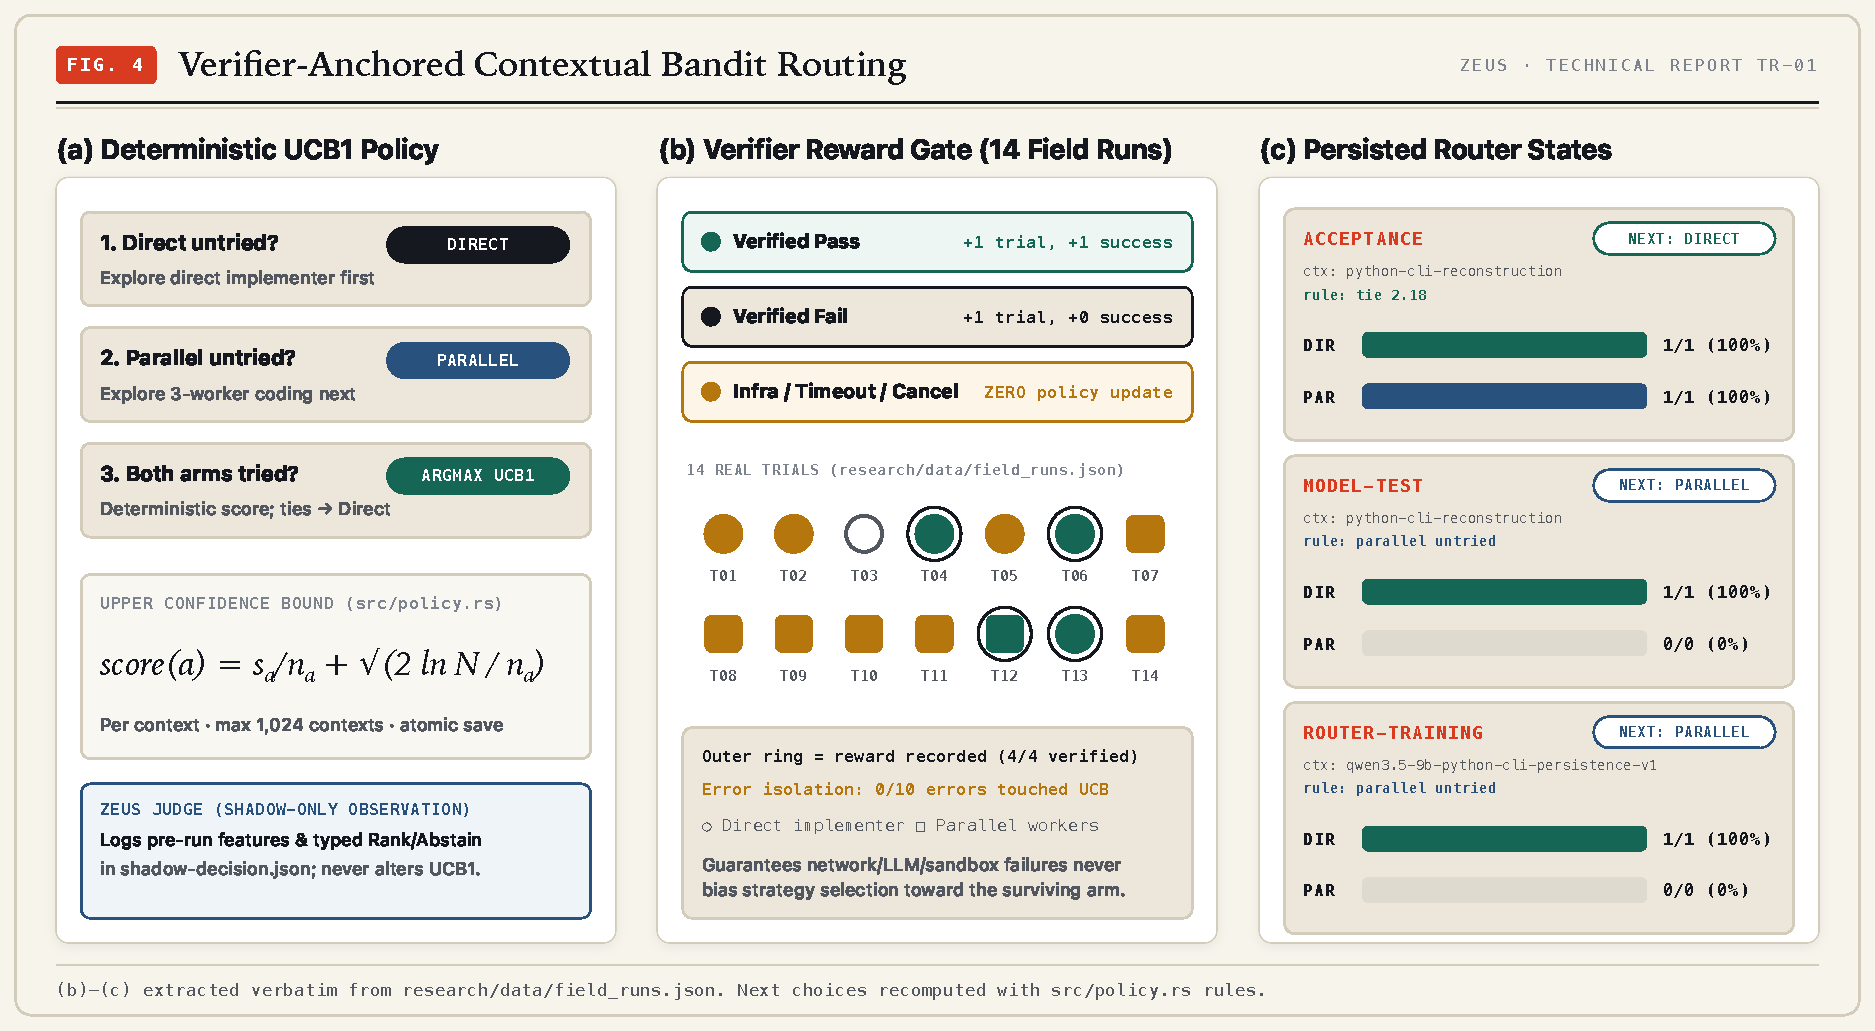
\includegraphics[width=\textwidth]{figures/fig4-routing.pdf}
  \caption{Deterministic UCB1 policy and verifier reward gate (\code{src/policy.rs}). Across all $14$ empirical field trials, only verified outcomes (outer rings on $T04$, $T06$, $T12$, $T13$) updated router counts; $0/10$ transport, planner-format, capability, or path-contract failures touched UCB weights.}
  \label{fig:routing}
\end{figure}

Crucially, UCB1 updates are gated strictly by external verification results (Figure~\ref{fig:routing}). A verified pass adds $(+1 \text{ trial}, +1 \text{ success})$; a verified functional failure adds $(+1 \text{ trial}, +0 \text{ success})$; transport timeouts, planner JSON syntax errors, unknown tool calls, path rejections, and user interrupts leave $n_c(a)$ and $s_c(a)$ untouched. Without this isolation, fragile infrastructure failures on one arm would permanently inflate the empirical win rate of whichever strategy ran under healthier network conditions.

% ==============================================================================
\section{Empirical Field Trials and Hardening Trajectory}
\label{sec:trials}

During initial runtime construction (November~1--3), $14$ exploratory local runs (\code{T01}--\code{T14}) were executed using Qwen~3.5-9B against a deterministic Python key-value store reconstruction fixture (\code{kv.py}, growing from $77$ to $82$ verification assertions). All run manifests and policy files were scrubbed of local paths into \code{research/data/field\_runs.json}.

\begin{figure}[htbp]
  \centering
  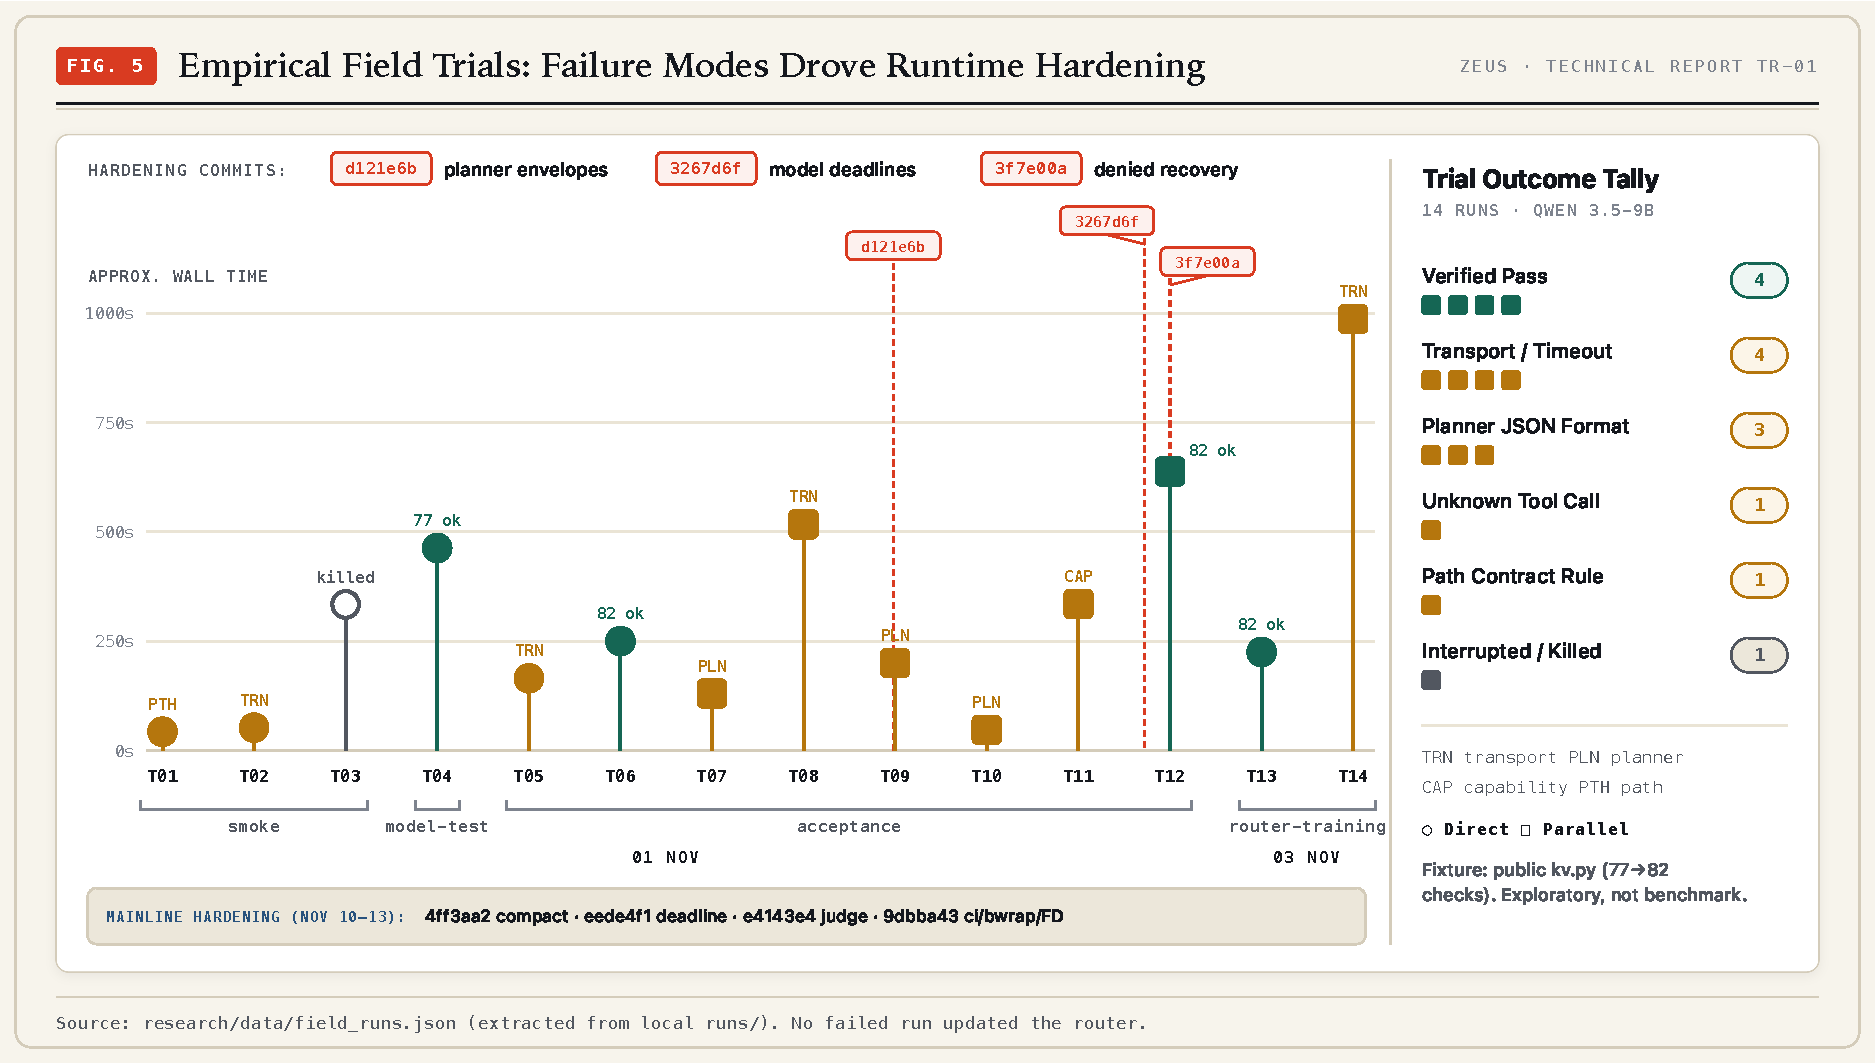
\includegraphics[width=\textwidth]{figures/fig5-field-trials.pdf}
  \caption{Chronology of all $14$ exploratory Qwen~3.5-9B field trials (\code{T01}--\code{T14}) extracted verbatim from local \code{runs/}. Every infrastructure failure class catalyzed concrete runtime fixes rather than polluting router state.}
  \label{fig:trials}
\end{figure}

Figure~\ref{fig:trials} reveals two findings:
\begin{enumerate}[leftmargin=1.5em,itemsep=2pt,topsep=2pt]
  \item \textbf{Observed runtime bottlenecks drove concrete engineering commits}: early path-contract failures (\code{T01}) and strict JSON planner errors (\code{T07}, \code{T09}, \code{T10}) led to planner JSON envelopes (\code{d121e6b}); sluggish multi-minute model stalls led to per-request deadlines (\code{3267d6f}); denied-action confusion led to typed error feedback (\code{3f7e00a}), immediately preceding parallel success \code{T12} ($82/82$ assertions passed). Subsequent hardening (\code{b9d4a4a}--\code{e4143e4}, plus CI \code{bubblewrap}/FD hygiene in \code{9dbba43}) targeted HTTP retries, compaction, whole-job deadlines, secret withholding, shadow scoring, and sandbox boundary enforcement.
  \item \textbf{Router invariance held under stress}: despite $10$ incomplete/infrastructure runs out of $14$ (due to Qwen~3.5-9B latency, local Ollama/LM transport timeouts, format errors, and manual cancellation on \code{T03}), \emph{zero} non-verified runs wrote policy state. In \code{acceptance}, both arms hold $1/1$ ($100\%$ verified); under the exact tie-breaking rule in \code{src/policy.rs} ($2.18 = 2.18$), Direct is deterministically chosen next, whereas \code{model-test} and \code{router-training} hold $1/1$ Direct and $0/0$ Parallel, cleanly selecting Parallel on the next execution.
\end{enumerate}

% ==============================================================================
\section{Deterministic Verification Corpus}
\label{sec:tests}

To decouple systems correctness from model availability, Zeus ships a static suite of $266$ \code{\#[test]} functions spanning $44$ integration test files under \code{tests/} plus $3$ inline unit tests in \code{src/runtime.rs} and $1$ unit test in \code{src/process.rs} ($46$ suites total; $2$ tests marked \code{\#[ignore]} for explicit opt-in runs alongside OS-gated Seatbelt/\code{bubblewrap} checks).

Figure~\ref{fig:tests} details test allocation across nine subsystems, led by model protocol, retry, and compaction coverage ($58$ tests), workspace/secret/output guards ($40$), plugins/MCP/analyzers ($39$), sandboxes/verifier/interruption ($37$), and policy/judge/evidence checks ($30$). Dedicated process-safety tests assert clean file-descriptor hygiene, verifying that external verifiers do not inherit open host sockets or launch channels when spawned cleanly.

\begin{figure}[htbp]
  \centering
  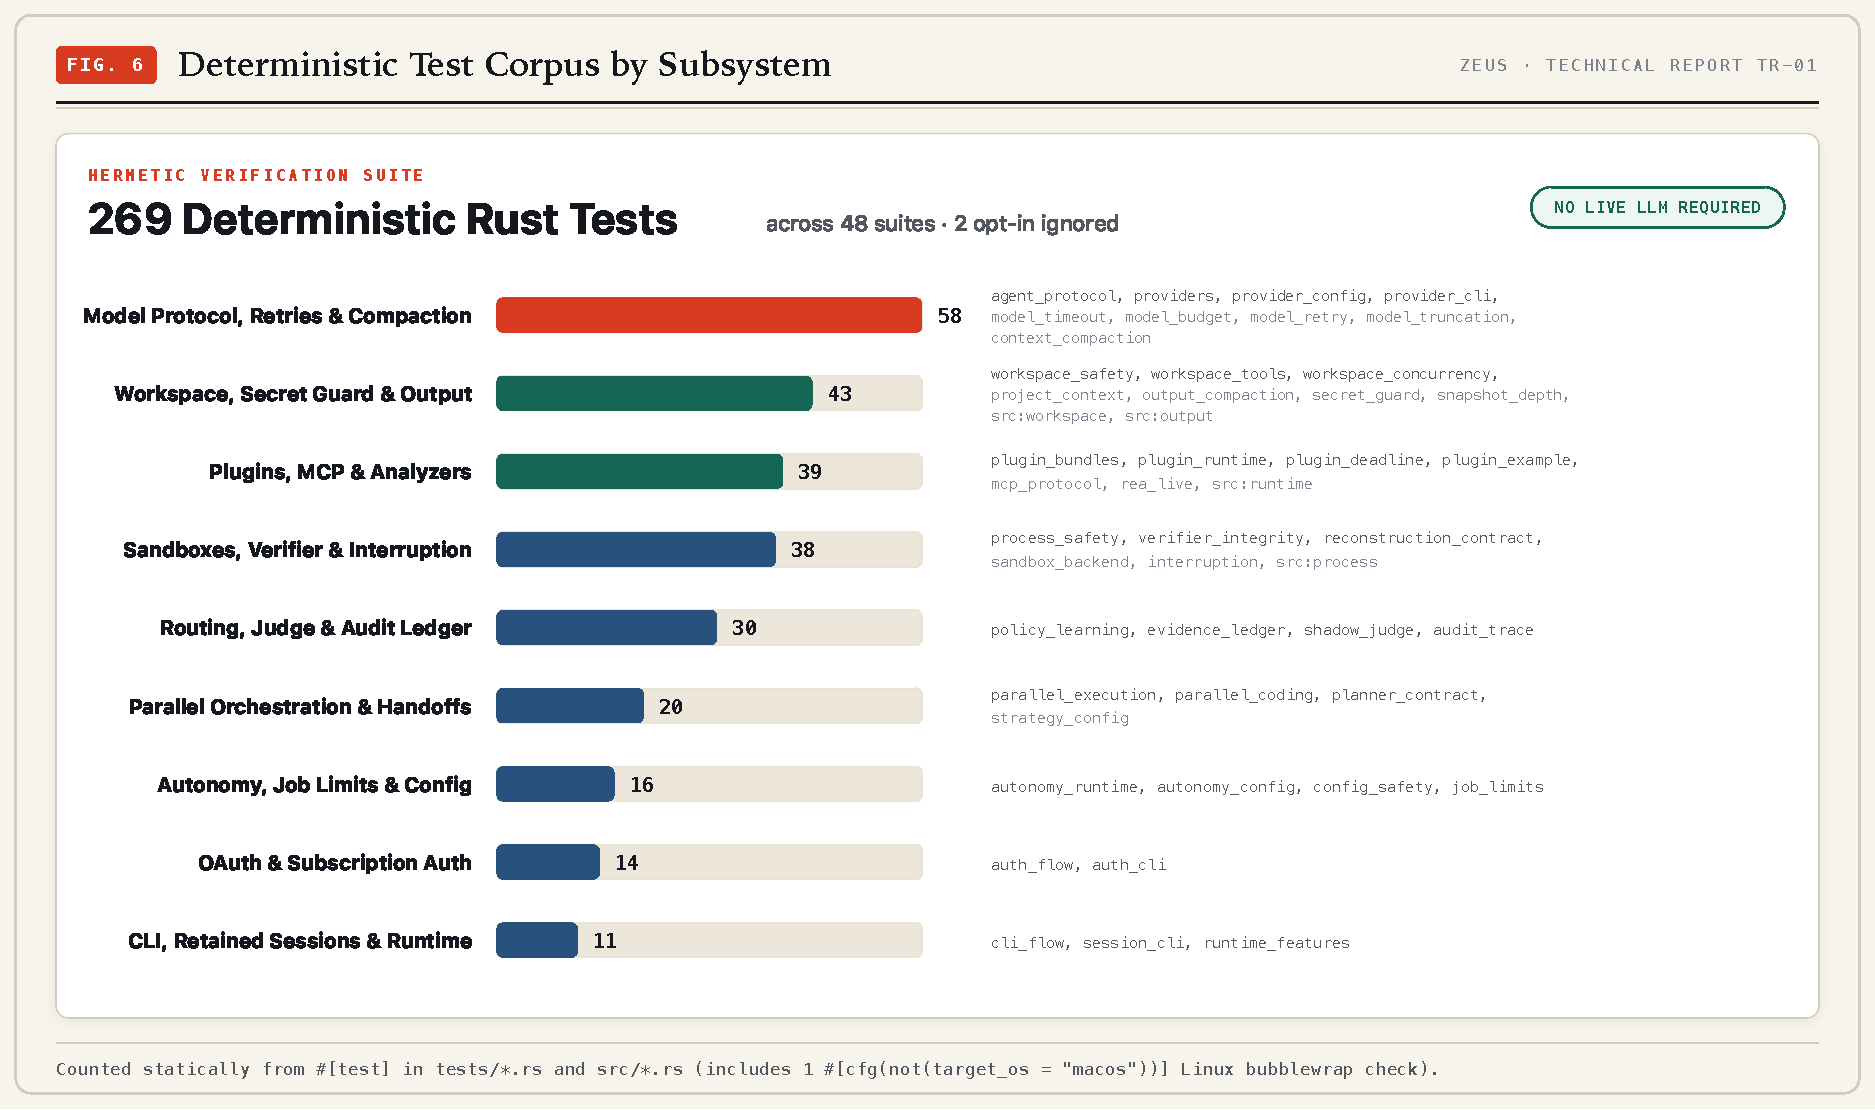
\includegraphics[width=\textwidth]{figures/fig6-tests.pdf}
  \caption{Static breakdown of Zeus's $266$ deterministic Rust tests grouped into nine architectural subsystems on revision \code{9dbba43}.}
  \label{fig:tests}
\end{figure}

% ==============================================================================
\section{Bounded Memory and Zeus Judge Shadow Abstention}
\label{sec:memory_judge}

Long coding trajectories fail abruptly when raw test logs or recursive file inspections overflow context limits (historically observed as provider rejections past $\sim 4$\,MiB). Mainline hardening between commits \code{abf3e7a} and \code{3b84f90} introduced three deterministic safeguards summarized in Table~\ref{tab:bounds}:
\begin{enumerate}[leftmargin=1.5em,itemsep=2pt,topsep=2pt]
  \item \textbf{Deterministic Tool-Result Compaction (\code{src/agent.rs})}: once prompt bytes cross \code{compaction\_threshold\_bytes} (default $1$\,MiB, floor $64$\,KiB) or on recoverable provider overflow, Zeus replaces older tool results in-place with \code{\{"elided":true\}} while unconditionally preserving the most recent $\code{PROTECT\_LAST\_TOOL\_RESULTS} = 4$ tool outputs (Figure~\ref{fig:judge}, right). Because edits operate reversibly over exact JSON markers and log an audit event, the model can re-read any compacted file rather than relying on lossy LLM summarization.
  \item \textbf{Bounded Handoff Projection (\code{src/output.rs})}: after all parallel workers join, raw worker outputs still stream verbatim to \code{events.jsonl}, while the integrator prompt receives \code{worker\_handoff} capped at $8{,}192$\,B per worker using an asymmetric $75\%$ head / $25\%$ tail UTF-8-safe split separated by \code{\textbackslash n[zeus: middle omitted]\textbackslash n}. Even across the maximum $12$ subtasks, integrator aggregation stays capped around $96$\,KiB.
  \item \textbf{Transient Retry Classification \& Whole-Job Deadlines (\code{src/model.rs}, \code{src/cancel.rs})}: HTTP transport timeouts and transient status codes trigger bounded retries with explicit classification, while whole-job deadlines and token ceilings halt runaway loops predictably across planner, worker, and integrator phases.
\end{enumerate}

While UCB1 explores across coarse contexts, jobs vary substantially in task size and autonomy limits. Commit \code{e4143e4} introduces \emph{Zeus Judge} (\code{src/judge.rs}), an experimental offline-fitted dual-head linear/logistic outcome estimator that records counterfactual recommendations to \code{shadow-decision.json} and post-run outcomes to \code{shadow-outcome.json} without altering runtime routing. Each job is projected onto an 8-dimensional vector under schema \code{job\_limits\_v1}:
\begin{equation*}
x = \Big[
\frac{|\text{task}|}{32768},\;
\frac{\text{max\_turns}}{32},\;
\frac{\text{max\_repairs}}{8},\;
\frac{\text{max\_calls}}{1024},\;
\mathbf{1}_{\text{calls}},\;
\frac{\ln(1 + \text{max\_tokens})}{\ln(1 + 2^{64}-1)},\;
\mathbf{1}_{\text{tokens}},\;
\frac{\text{max\_job\_s}}{86400}
\Big],
\end{equation*}
bound cryptographically via $\text{SHA-256}(\{\text{context}, \text{model}, \text{protocol}, \text{endpoint}, \text{verifier}\})$.

\begin{figure}[htbp]
  \centering
  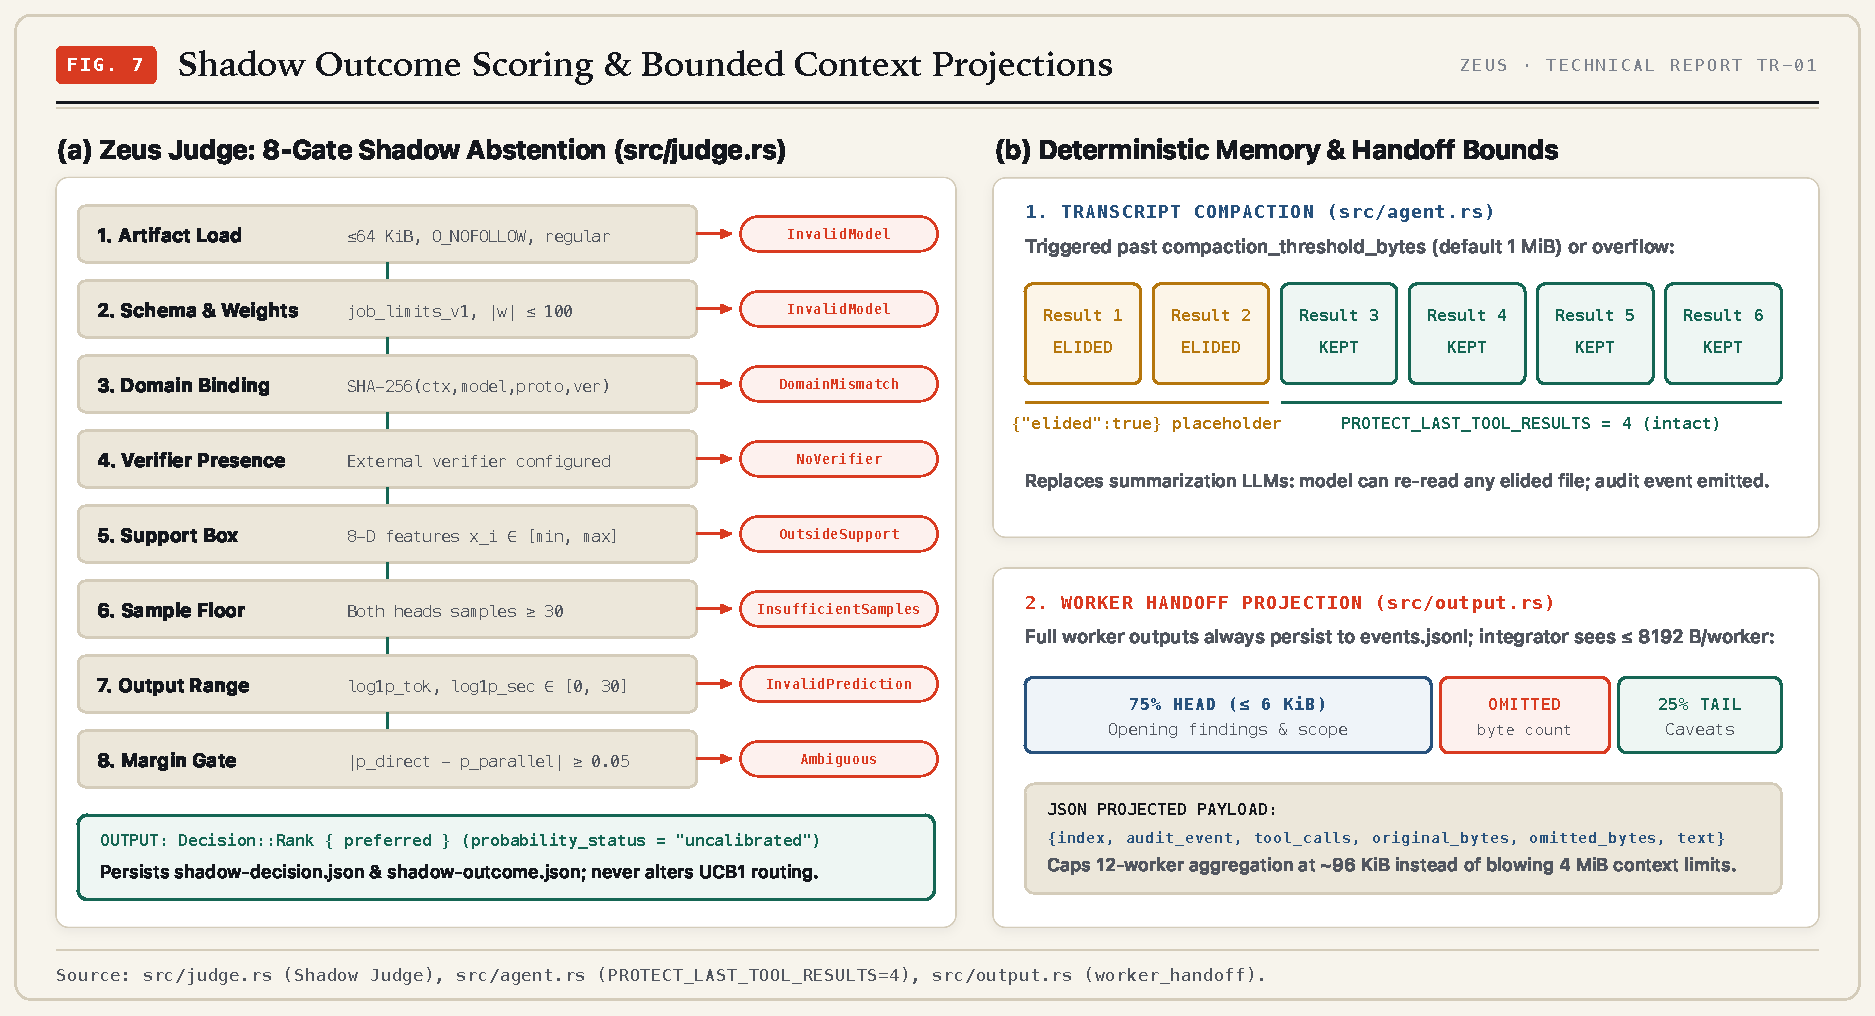
\includegraphics[width=\textwidth]{figures/fig7-judge-handoffs.pdf}
  \caption{Left: 8-gate fail-closed abstention pipeline in \code{src/judge.rs}, preventing uncalibrated or out-of-domain artifacts from producing a preferred strategy rank. Right: deterministic transcript compaction and bounded worker handoff projections.}
  \label{fig:judge}
\end{figure}

As shown in Figure~\ref{fig:judge} (left), \code{judge::evaluate} must clear eight sequential integrity gates before returning \code{Decision::Rank}: (1) artifact read via \code{O\_NOFOLLOW} regular file $\le 64$\,KiB, (2) schema \code{job\_limits\_v1} with finite weights $|w| \le 100$, (3) exact domain SHA-256 equality, (4) external verifier presence, (5) support box containment $x_i \in [\min_i, \max_i]$, (6) sample floor $n_{\text{samples}} \ge 30$ on both heads, (7) finite predicted $\log(1 + \text{tok})$ and $\log(1 + \text{sec})$ in $[0, 30]$, and (8) pairwise decision margin $|p_{\text{direct}} - p_{\text{parallel}}| \ge 0.05$. Even when ranked, probability outputs explicitly carry \code{probability\_status = "uncalibrated"}.

% ==============================================================================
\section{Conclusion}
\label{sec:conclusion}

Zeus demonstrates that reliability gaps in agentic coding stem largely from missing OS, concurrency, and contract boundaries rather than insufficiently persuasive system prompts. By keeping candidate snapshots secret-free, forcing pre-admission disjointness across at most three work-conserving workers, projecting integrator handoffs into bounded $8$\,KiB envelopes, isolating adaptive routing updates behind sandboxed verification, and wrapping learned outcome models inside eight fail-closed abstention gates, Zeus turns nondeterministic LLM completions into auditable, restart-safe systems behavior. Future empirical work requires held-out software benchmarks spanning stronger frontier and local models, cross-platform field trials on Linux \code{bubblewrap} hosts, and collecting $\ge 30$ samples per head to graduate Zeus Judge from abstention into calibrated active evaluation.

% ==============================================================================
\begin{thebibliography}{9}

\bibitem{auer2002ucb1}
P.~Auer, N.~Cesa-Bianchi, and P.~Fischer.
\newblock Finite-time analysis of the multiarmed bandit problem.
\newblock \emph{Machine Learning}, 47(2--3):235--256, 2002.

\bibitem{graham1969bounds}
R.~L. Graham.
\newblock Bounds on multiprocessing timing anomalies.
\newblock \emph{SIAM Journal on Applied Mathematics}, 17(2):416--429, 1969.

\bibitem{zeusarch}
V.~Viswanath.
\newblock Zeus Implementation Contract and Ancestor Provenance (\code{ARCHITECTURE.md}, inspecting \emph{Hermes} \code{bf0203a7}/\code{c419cf7c} and \emph{Prime} \code{c4c238ca}/\code{c6d4da94}), 2026.

\bibitem{zeusjudge}
V.~Viswanath.
\newblock Zeus Judge Shadow Outcome Contract (\code{docs/JUDGE.md}, \code{src/judge.rs}, rev. \code{9dbba43}), 2026.

\bibitem{bwrap}
Project Atomic / Containers.
\newblock \emph{bubblewrap}: unprivileged sandboxing tool for Linux namespaces.
\newblock \url{https://github.com/containers/bubblewrap}.

\end{thebibliography}

\end{document}
